\subsection*{Hierarchy of Roles\label{sec:hierarchy-of-roles}}


In an ideal situation, sufficient depth and breath for decision making would be embodied in one person. That might not be possible in every situation. One way to resolve this is to identify distinct scopes of responsibility and then assign different members of an organization separate scopes for decision making. Within a decision making scope there may be more work than one person can handle, so a team is formed. That team may have some members focused on tactical work and other members focused on strategy and coordination. Hierarchy within an organization is the formalization of separate decision-making scopes and associated specialization. 

Partitioning knowledge and decision making enables complex work beyond what one person can accomplish and causes friction among members. An expert reporting to a manager knows things the manager does not, and the manager may have context that the expert lacks. Both bureaucrats (the expert and the manager) need to convey their respective understanding and seek the holistic view.

Hierarchical decision making is one option for coordination among alternatives (like consensus), so why is hierarchy so common? Members of an organization gravitate towards hierarchy because it helps define task scope, assigns responsibility, and obviates a need for building consensus. Reaching consensus for every decision would take time and be more burdensome than appointing a person as the decision maker.

\ \\

A hierarchical organization with partitioned knowledge introduces a challenge: the order in which you share information with others matters. Your choices for who to first describe an idea to are your peers, your management, and your subordinates. 
\marginpar{[Tag] Trilemma} 
\index{trilemma!communication priority: peers, management, subordinates}
The people subordinate to you know more about the topic and are exposed to the consequences. Giving them a chance to vet the idea results in a more robust idea and validates their value in the organization. Alternatively, first sharing your idea with management  allows your superiors to provide context you might not be aware off. And choosing to first start the conversation with your peers indicates you value the relationship and decreases the risk of duplicating work.

\ \\

I've included hierarchy in the section on Fundamentals of Bureaucracy, but that does not imply that hierarchy is a required feature of bureaucracy. Hierarchies of bureaucrats are a common \href{https://en.wikipedia.org/wiki/Organizational_structure}{organizational structure} and are worth studying even if not essential to bureaucracy. The relevance of understanding hierarchy is to identify recurring behavior and patterns to leverage.
Organizations of bureaucrats can intentionally work against the use of hierarchy for decisions, but the amount of effort needed to enable alternatives results in hierarchy being a common approach.

The benefits of formal hierarchy include improved capacity for the number of policy decisions made, enabling consistency of decisions, and leveraging specialization of knowledge. 
Hierarchical decision making has costs: higher latency (compared to a single decider), inconsistency among bureaucrats (dissemination isn't perfect), waste due to inefficiency, and 
\hyperref[sec:unavoidable-hazards]{many others}.
\ifsectionref
described in section~\ref{sec:unavoidable-hazards}. 
\fi
As another example of the potential for harm, hierarchy enables strategic ignorance. Bureaucrats in positions of power can deny having knowledge of improper activity\footnote{L.~McGoey, ``The Unknowers: How Strategic Ignorance Rules the World" (2019)
% review: https://www.tandfonline.com/doi/abs/10.1080/19460171.2020.1768422?journalCode=rcps20
and 
L.~McGoey, ``The logic of strategic ignorance" (2012). DOI 
10.1111/j.1468-4446.2012.01424.x
}. Whether that is a problem or benefit depends on your role. 



The structure of an organization is dynamic, but at each point in time an organization typically has a defined set of roles. Each role is distinguished by different scopes of decision authority. 
Roles are often confused with titles. What matters is the role (scope of decisions) and who reports to whom. The names of teams can be similarly not descriptive.




Roles in an organization are defined by the boundaries of responsibility. The purpose of a role is to minimize conflict, decrease the need for coordination, reduce redundancy, and allow for control of resources. Clear boundaries of responsibility  enable effective bureaucracy. 


A conventional characterization of an organization's hierarchy involves two criteria: the depth and breadth of the \gls{org chart}.
The more people a supervisor oversees, the flatter the organization -- that's the breadth of the organization. The depth of the hierarchy is how many layers there are. See the Valve handbook~\cite{2012_Valve} and Joreen's essay~\cite{1972_Joreen} for contrasting views on the merits of an organization's hierarchy. 

A more practical view of an organization's hierarchy also involves two criteria. The two choices of how a hierarchy is shaped are 
1) how many people a supervisor oversees and 
2) how many supervisors a person has. 
You might naively expect that an employee has one boss, but that is \href{https://en.wikipedia.org/wiki/Matrix_management}{not a requirement}. A supervisor for a given topic may have many people reporting to them, and a bureaucrat with multiple roles may report to more than one supervisor.

\ \\

Acting as part of a group means ceding part of your autonomy. Hierarchy cedes some of your responsibility and adds expectations about relationships.
The consequence of hierarchy in an organization is that, as a member of the bureaucracy, you do not have full autonomy -- otherwise you would not be a member of the hierarchy. At the same time, you are not under strict control of the organization -- you still have some subjective decision making authority as a bureaucrat.

The person at the top of the hierarchy does not know everything. The person at the top of the hierarchy does not have input on every decision made in the organization. Some autonomy is retained by all members of the bureaucracy.

Independent of the defined roles and titles in an organization's hierarchy, there are a set of implicit roles and a separate social hierarchy of informal influencers and decision makers. Informal influencers in a bureaucracy usually have long relationships with the decision maker or relevant credentials or both. The credentials can be formal (e.g., a \href{https://en.wikipedia.org/wiki/Doctor_of_Philosophy}{PhD}) or informal (demonstrated success on a project). In either case, the decision maker is relying on another person's expertise. 

Another set of informal relationships within an organization is mentors and mentees. These relations allow mentors to share institutional knowledge to mentees, and allow people in senior positions to access the novice perspective. 


\ \\

One consequence of hierarchy is a sense of fear felt by people who report to other people. This fear stems from the loss of control (less autonomy) that leaves the person feeling disempowered. 

For example, consider the following relationship. Sue is perceived to have power over another person, Amy, because Amy gave up some control to Sue. Amy not having full control over decisions triggers the feeling of fear in Amy, regardless of how Sue behaves. Having complete responsibility for decisions also induces anxiety.

\begin{figure}[H]
    \centering
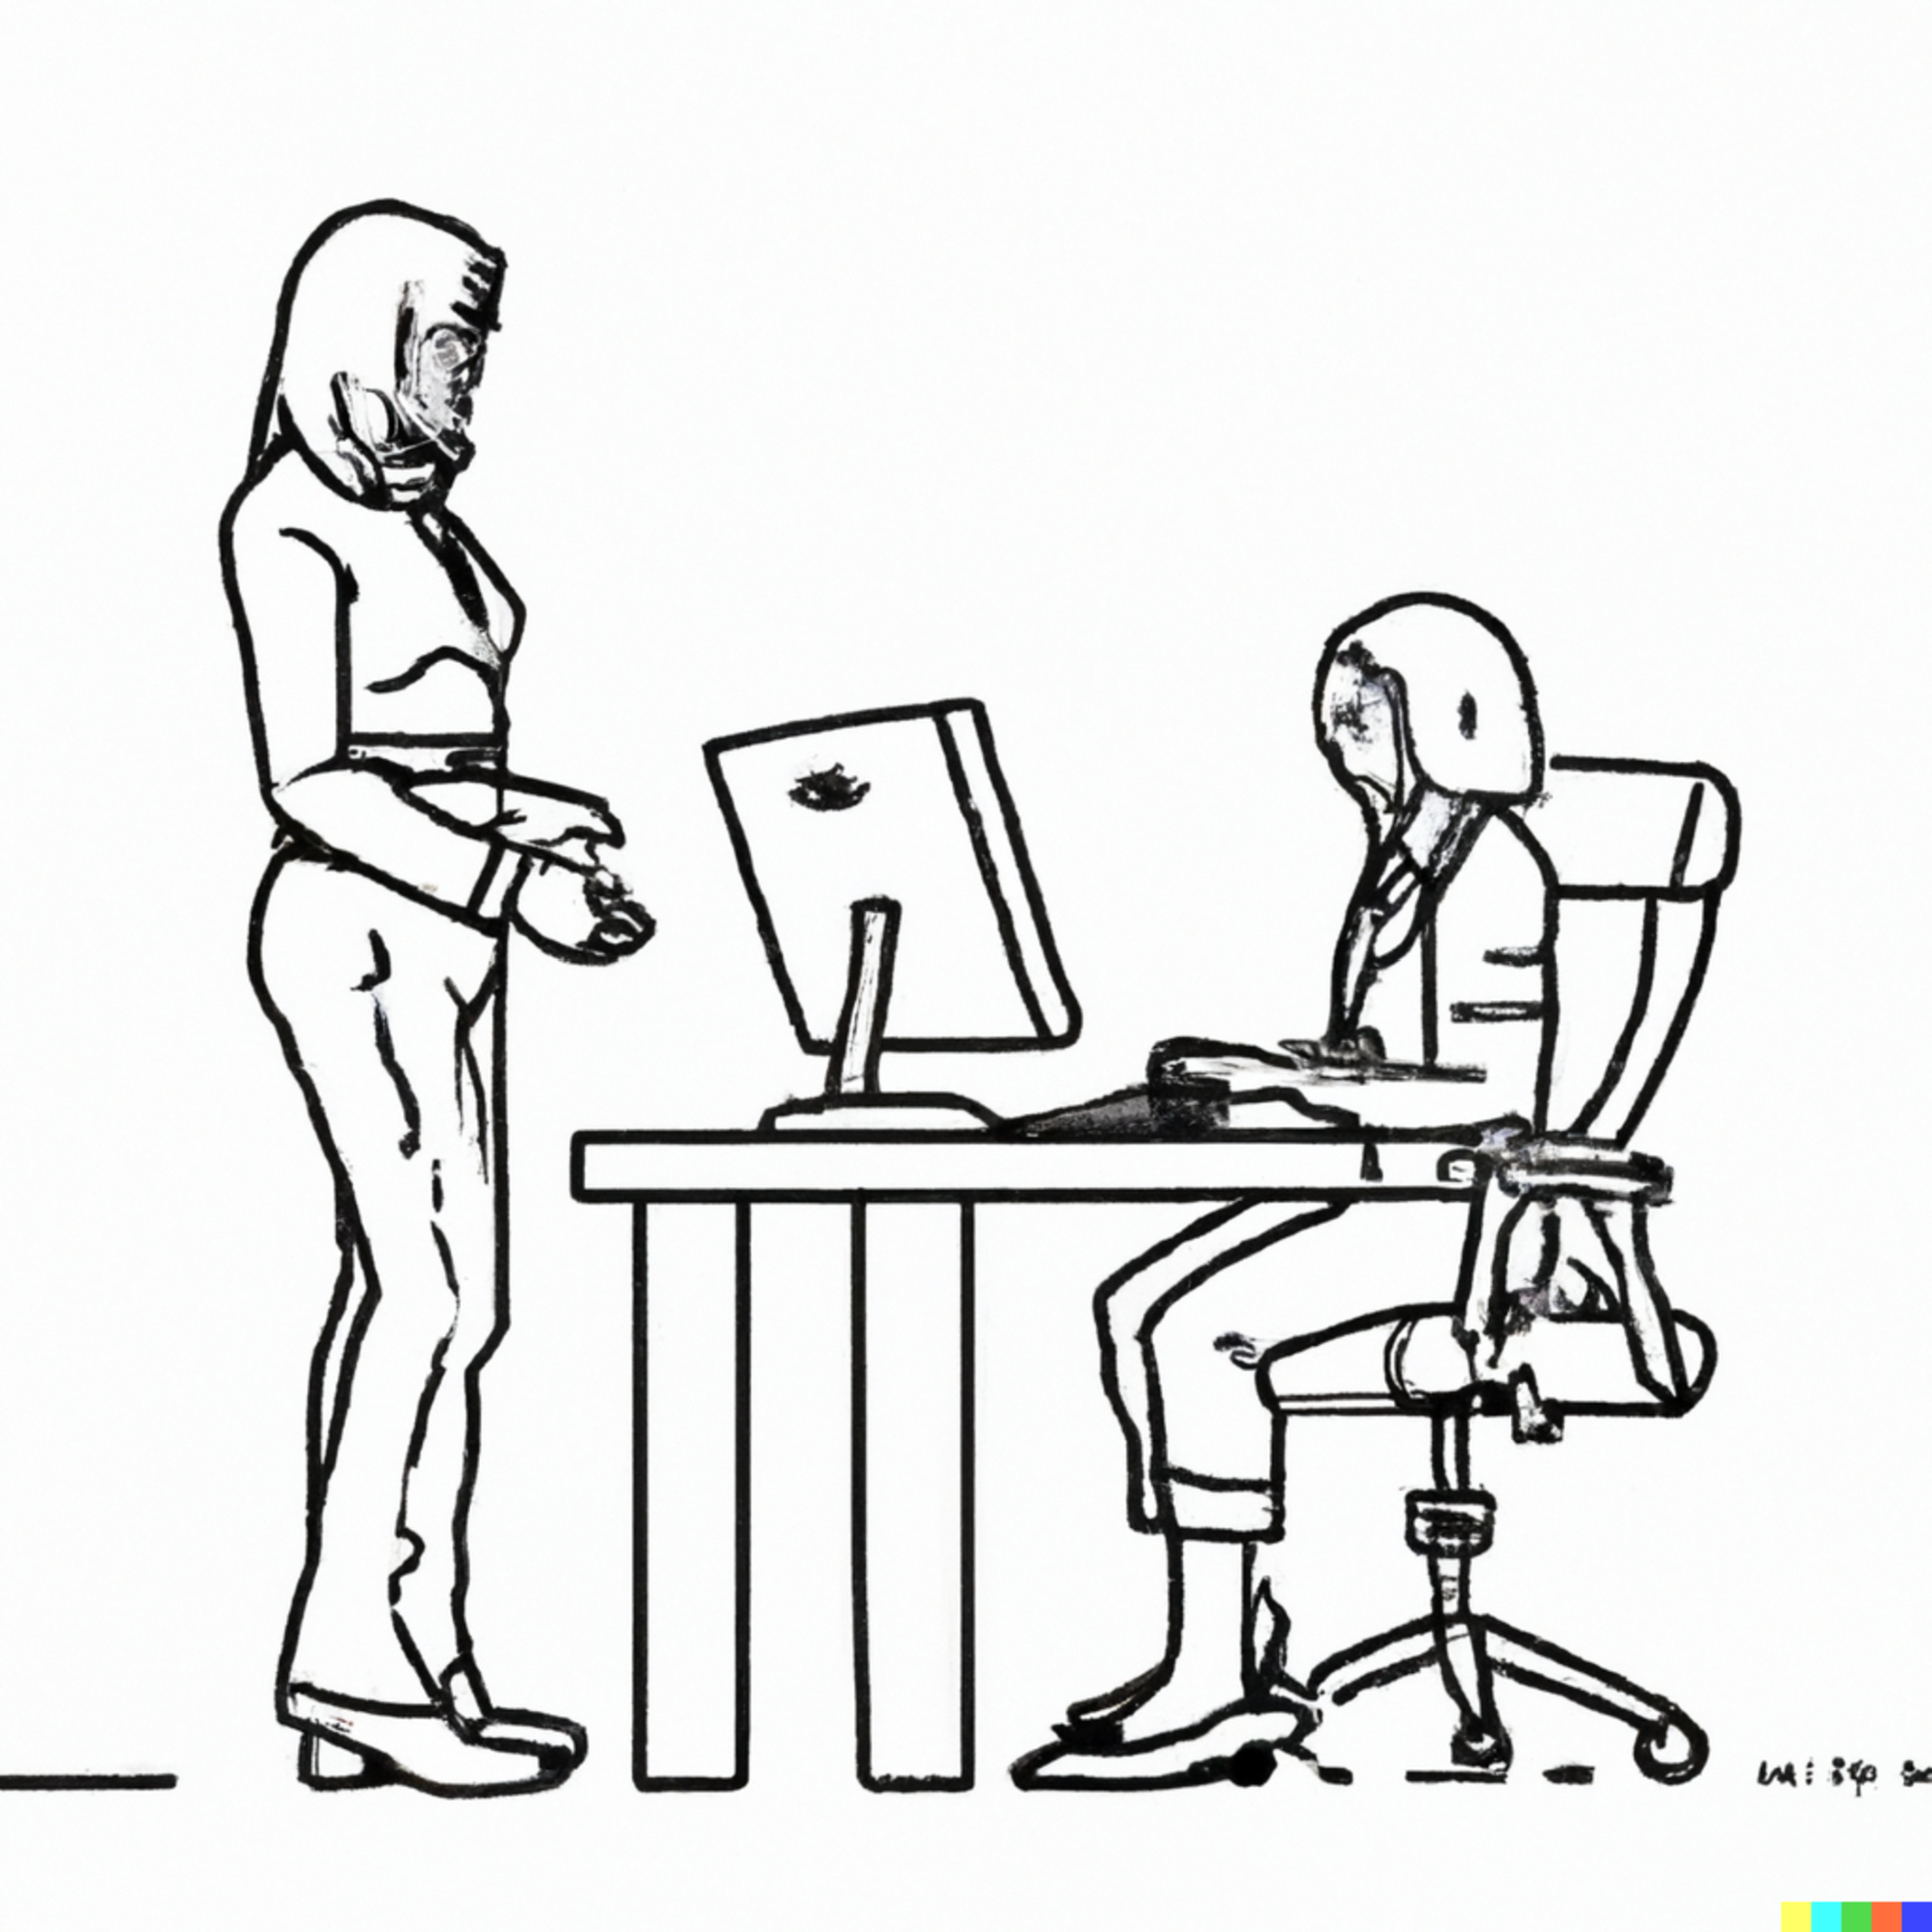
\includegraphics[width=0.6\textwidth]{images/female_supervisor_standing_while_talking_to_seated_female_employee_typing_on_keyboard.pdf}
    \caption{Sue and Amy.}
    \label{fig:subordinate_and_supervisor}
\end{figure}



If Sue is aware of the potential for this emotional experience, Sue can compensate for Amy's fear by being friendly and receptive towards Amy. Alternatively Sue may exploit or rely on the fear felt by subordinates. Sue not noticing or accounting for Amy's fear does not invalidate Amy's emotional experience.


% Active bystander when the person doing wrong is in a position of authority
% PACT (Probe, Alert, Challenge, Take Action)
% https://mobile.twitter.com/GeorgetownABLE/status/1408498438203969541


% Mintzberg's Coordination Mechanisms
% https://www.youtube.com/watch?v=IZET8VjSifQ

